\section{Ray marching}
\begin{frame}{Algoritmos basados en rayos}
En realidad esta es un familia de algoritmos, los mas importantes son:

\begin{itemize}
    \item \href{https://en.wikipedia.org/wiki/Ray_casting}{Ray Casting:} El primero en ser desarrollado. Consiste en lanzar un rayo por cada pixel del viewport. Para ver donde interfecta la escena.
    \item \href{https://en.wikipedia.org/wiki/Ray_tracing_(graphics)}{Ray Tracing:} Una generalización donde cada vez que se intersecta la escena, se calcula el angulo de reflexión y se continua siguiendo el rayo, hasta cumplir algún criterio de paro.
    \item \href{https://en.wikipedia.org/wiki/Ray_marching}{Ray Marching:} Una forma de usar la sdf, para acelerar el camino de los rayos de manera recursiva. Este es el mas usado en ShaderToy
    \item \href{https://en.wikipedia.org/wiki/Path_tracing}{Path Tracing:} En vez de lanzar un rayo, se lanzan varios rayos a ángulos muy similares usando el método de Monte Carlo.
\end{itemize}

\end{frame}

\begin{frame}{El rayo}
\begin{block}{Rayo}
Un rayo es el semisegemento de linea $\mathbf{r}(s) = \mathbf{o} + s  \mathbf{d}$, donde $s \in \mathbf{R}^{+}$ es un escalar positivo, $\mathbf{o}$ es un punto en $\mathbb{R}^3$ y $|\mathbf{d}| = 1$ un vector unitario en $\mathbb{R}^3$. 

\end{block}

\begin{columns}
\column[t]{0.5\textwidth}
\begin{itemize}
    \item $\mathbf{o}$ es el origen del rayo.
    \item $\mathbf{d}$ es la direccion del rayo.
    \item $s$ es el parámetro.
\end{itemize}    
\column[t]{0.5\textwidth}
\begin{figure}[htp]
    \centering
    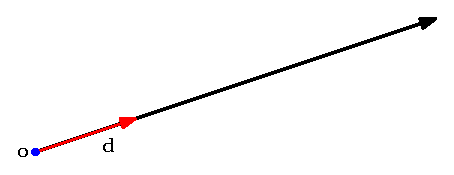
\includegraphics[width=0.6\textwidth]{img/ray}    
\end{figure}
\end{columns}
\end{frame}

\begin{frame}{Ray Marching}
Es una técnica para hacer un avance adaptativo de lo rayos.
\begin{enumerate}
    \item En el punto actual del rayo calcula la distancia $d$ del punto con respecto a la escena.
    La \emph{distancia} de la escena, es la minima de todas las sdfs a las figuras en la escena.
    \item Si $d$ es menor que un cierto $\epsilon$, termina y reporta que hay una colison con la escena.
    \item Si $d$ es mayor que un cierto valor frontera termina y di que no hay colision.
    \item Avanza el rayo en $d$ unidades, y repite desde 1.
\end{enumerate}
Esta técnica solo se puede usar si\ldots
\begin{itemize}
    \item Definimos la escena por medio de sdfs.
    \item El rayo tiene un vector de dirección unitario.
    \item Las sdf están bien definidas:
    \begin{itemize}
        \item Continuas
        \item La distancia esta en la misma dimensión que la escena.
    \end{itemize}    
\end{itemize}

\end{frame}

\begin{frame}{Ray Marching: una imagen}

\begin{itemize}
    \item En la practica se pone un numero máximo de pasos como criterio extra de paro.
\end{itemize}    

\begin{figure}[htp]
    \centering
    \includegraphics[width=0.6\textwidth]{img/rayMarch}    
\end{figure}

Hay un \href{https://www.shadertoy.com/view/4dSfRc}{ejemplo} para visualizar la técnica en ShaderToy mismo.

\end{frame}

\begin{frame}[fragile]{Ray Marching: en código}
\begin{listing}
\begin{minted}{glsl}
float rayMarch(Ray ray, float start, float end) {
  float depth = start;

  for (int i = 0; i < MAX_MARCHING_STEPS; i++) {
    vec3 position = ray.origin + depth * ray.direction;
    float d = sdScene(position);
    depth += d;
    if (d < PRECISION || depth > end) break;
  }

  return depth;
}
\end{minted}
\end{listing}

\end{frame}

\begin{frame}{Visualizar en 3D}
\begin{itemize}
    \item Para no ver todo de un color plano en 3D, necesitamos hacer shading.
    \item Para hacer shading, necesitamos (entre otras cosas), la normal $\mathbf{n}$ a la superficie en el punto de contacto.
    \item Podemos utilizar la misma sdf, para calcular el gradiente $\nabla$ de la figura. El gradiente es una buena aproximación a la normal: $\nabla \approx \mathbf{n}$.
\end{itemize}
$$\nabla (f(\mathbf{x})) = \begin{pmatrix}
f(x + \epsilon, y, z) - f(x - \epsilon, y, z)\\
f(x, y + \epsilon, z) - f(x, y - \epsilon, z)\\
f(x, y, z + \epsilon) - f(x, y, z - \epsilon)
\end{pmatrix}$$
Donde $f(\mathbf{x})$ es una sdf y $\epsilon$ un numero positivo muy pequeño.
\begin{itemize}
    \item Finalmente, si definimos una fuente de luz, con una posición $\mathbf{l}$ en la escena.
    \item Una forma muy sencilla de shading puede ser: $c = \max(\mathbf{k}_d (\mathbf{l} \cdot \mathbf{n}), \mathbf{0})$.
    \item Donde $\mathbf{c}$ es el color resultante y $\mathbf{k}_s$ es el color predominante de la superficie.
\end{itemize}
\end{frame}

\begin{frame}{Ejercicio: Esfera usando Ray Marching}
\url{https://github.com/nemediano/tallerShadertoy/tree/main/codigo/Ejercicio4}
\begin{columns}
\column[t]{0.5\textwidth}
     \begin{itemize}
         \item De momento usa solo una esfera en la escena
         \item Trata de definir tu cámara, la esfera y una fuente de luz, en lugares sencillos respecto al origen.
         \item De momento usa la reflexión difusa, para que puedas visualizar al esfera
         \item Puedes usar el código de comienzo de la escena para empezar.
     \end{itemize}
\column[t]{0.5\textwidth}
        \begin{figure}[htb]
            \centering
            \includegraphics[width=0.6\textwidth]{img/Ejer4}
        \end{figure}
\end{columns}
\end{frame}
